\documentclass[10pt,journal,compsoc]{IEEEtran}
\usepackage[utf8]{inputenc}
\usepackage[T1]{fontenc}
\usepackage{graphicx,booktabs,amsmath,url}
\usepackage[hidelinks]{hyperref}
\hyphenation{Rum-mi-kub}

%% Repositorio anonimo: cole aqui a URL que o anonymous.4open.science devolve
%% (ele anonimiza o nome do dono e do repo, e espelha a branch revisao-anonima).
\newcommand{\repoanon}{\url{https://anonymous.4open.science/r/rummikub}}

\begin{document}

\title{What Does It Mean to Win? Metric Choice Reverses the Strategy Ranking in Rummikub}
\author{}
\markboth{IEEE Transactions on Games}{}
\IEEEtitleabstractindextext{%
\begin{abstract}
We study which simple strategy wins at two-player Rummikub, and find that the answer depends on how winning is measured. In a simulator of the official rules, a paired round-robin of seven interpretable strategies is won by the \emph{joker-saver}, which plays as many tiles as possible but spends a wildcard only to empty its hand. Four ablations ($13{,}000$ games) isolate the cause: forbidding the joker as the final tile reverses the advantage, and $71\%$ of the saver's wins end with a joker. Official Rummikub, however, is zero-sum in tile points, with a joker left in hand counting $30$. Scoring the same $18{,}000$ games both ways, the saver is first in games won and sixth of ten in points. Over sessions of ten hands with accumulated points, the format the rules define, the inversion is complete: the saver wins the most hands of any strategy and the fewest sessions, losing $72.5\%$ of sessions to max-tiles, and the session ranking is the exact reverse of the per-hand win ranking. A per-hand win rate of $0.573$ corresponded to losing three sessions in four. Twenty-five learned and search agents, including PPO, Deep Monte Carlo, a determinised search given the true hidden hands, training on the official reward, per-decision potential shaping, and training on the session outcome while seeing the running balance, fail to beat the best heuristic under either metric. Scaling the training budget $27\times$ to $576{,}000$ games produces the first learned agent to beat the champion in points ($+4.69$ $[+2.10,+7.28]$), and it does so by \emph{winning fewer hands} and losing more cheaply; over thirty independent training seeds a $48{,}000$-game recipe still trails the best heuristic by $0.89$ $[0.51,1.26]$ points per hand. A paired tournament against a fixed strong field confirms the pattern at three and four players, where the best heuristic's edge shrinks and vanishes ($-0.0005$ $[-0.0082,+0.0072]$ at four), and scaling a \emph{win}-reward agent to $192{,}000$ games against a league that never includes that heuristic makes it worse, not better, so the best Rummikub player here remains a three-line rule.
\end{abstract}
\begin{IEEEkeywords}
Game AI, imperfect information, evaluation metrics, reinforcement learning, benchmark design, Rummikub.
\end{IEEEkeywords}}
\maketitle
\IEEEdisplaynontitleabstractindextext
\IEEEpeerreviewmaketitle

\section{Introduction}
\IEEEPARstart{R}{ummikub} is a tile game in which players empty their hands by forming runs and groups on a shared table. Its \emph{optimisation} subproblems are well studied: forming the best set of melds from a hand is polynomial-time solvable but becomes hard under generalisations \cite{vanrijn2016}, and integer linear programming solves full table-rearrangement problems \cite{denhertog2006}. Much less is known about which \emph{playing policies} win more often. Popular advice (``keep your jokers'') is widespread but, to our knowledge, untested.

This paper reports a result that began as a strategy study and became a measurement study. We first confirm the folk advice in its conditional form and explain it mechanistically: among seven interpretable strategies, the one that hoards wildcards until they can end the game wins the most games, and an intervention on that single exception reverses the effect. We then observe that the quantity we had been maximising --- games won --- is not the quantity the rules define. Official Rummikub is zero-sum in tile points, a joker left in hand counts $30$, and play is organised in sessions of several hands with accumulated scores. Re-scoring the same games, and then simulating sessions, reverses the ranking: the policy that wins the most hands wins the fewest sessions.

We ask four research questions.
\begin{description}\itemsep0pt
\item[RQ1] Among a menu of interpretable strategies, which wins most often?
\item[RQ2] What \emph{mechanism} explains the winner's advantage?
\item[RQ3] Does the answer survive the scoring metric printed in the rules, and the multi-hand format in which the game is played?
\item[RQ4] Can reinforcement learning (RL), a language-model decision-maker or a search agent beat the best fixed strategy, under either metric?
\end{description}

\paragraph*{Status of the evidence}
RQ1 is exploratory. RQ2 was designed after seeing the RQ1 result, with four competing explanations, and is corrected as one family; not pre-registered. The RQ3 experiments and the official-reward run of RQ4 fixed criteria and seeds in writing beforehand, and test seeds were spent once. All results are conditional on this simulator and menu; the supplement has per-game records and every analysis script.

\section{Related Work}
\paragraph*{Rummikub}
The literature we found treats Rummikub as an optimisation problem: a polynomial-time algorithm for the one-hand puzzle \cite{vanrijn2016}, an integer-programming formulation for rearranging the table \cite{denhertog2006}, a thesis counting winning hands \cite{feijen2023}, and one that reduces the solver's memory and classifies puzzle difficulty \cite{wekken2025}. The last explicitly notes that the multi-player game (initial meld, table manipulation, strategy) has received little study and leaves strategy for future work. We found no study evaluating learning or search agents on the full multi-player game against heuristic baselines; this is the result of a limited search, not a proof of absence. The closest learning study we know is on a sibling game: temporal-difference learning with self-play lost to co-evolution of the value function in gin rummy \cite{kotnik2003}.

\paragraph*{Learning in large-action card games}
DouZero reaches strong DouDizhu play by Monte Carlo returns, a network that scores encoded (state, action) pairs, and many parallel actors, which suits action sets that change from turn to turn \cite{zha2021}; our move network likewise scores concrete moves rather than using a fixed action head. Suphx adds global reward prediction and oracle guiding to deep RL for mahjong \cite{li2020}. Policy-gradient self-play against a pool of past checkpoints is common practice in tabletop-game RL \cite{balla2024}, which our league runs follow. A large-scale study finds generic PPO \cite{schulman2017} competitive with game-theoretic deep-RL methods in imperfect-information games \cite{rudolph2025}. Group-relative advantages, which replace a learned critic by standardising returns within a group of rollouts sharing a prompt, were introduced for language-model training \cite{shao2024}; we use the same estimator with a group of games sharing a deal. Our shaping term is a potential difference and therefore policy-invariant in the sense of \cite{ng1999}. The closest positive result to our own setup is IRumAI, which warm-starts PPO by behaviour cloning in Indian Rummy and reaches a $53.9\%$ win rate against the strongest search baseline unseen in training \cite{mohan2026}; our recipe is the same in outline (clone, then policy gradient) and does not reproduce that outcome, which we discuss in Section~\ref{sec:disc}.

\paragraph*{Search under hidden information}
Perfect-information Monte Carlo (PIMC) sampling, which our search agent follows, is practical but suffers strategy fusion, since the search may choose different continuations in worlds the player cannot distinguish \cite{frank1998}; its empirical success has been characterised \cite{long2010}, and information-set MCTS searches the player's information set instead of sampled worlds \cite{cowling2012}.

\paragraph*{Evaluation}
Our methodological conclusion is adjacent to work arguing that deep-RL comparisons rely too heavily on point estimates from few runs \cite{agarwal2021}, a critique of \emph{statistical} reliability at a fixed metric. We report a case where the metric itself, not its variance, reverses the conclusion.

\section{Simulator and Strategies}
\paragraph*{Game}
Two players in the main experiments; $106$ tiles ($4$ colours $\times$ values $1$--$13$ $\times$ $2$ copies, plus $2$ jokers); $14$ tiles per hand. A turn either draws one tile or lays tiles down. The first lay-down (the \emph{opening meld}) must be worth at least $30$ points using only the player's own tiles and may not touch the table. Afterwards a player may lay several melds, extend melds, and rearrange the whole table, provided every meld is valid at the end of the turn and at least one tile from the hand was played. The two jokers are shuffled with the other tiles. A hand ends when a rack is empty; if the pool is empty and all players pass in succession, it ends as well. Seat~0 moves first. The engine supports two to ten players and was validated against an independent third-party solver (Section~\ref{sec:rob}).

\paragraph*{Scoring}
Three rules appear in this paper. \textbf{Game count}: win $=1$, draw $=0.5$, loss $=0$, the convention we started with. \textbf{Official points} \cite{pagat2024}: the player who goes out scores the sum of all tiles left on opponents' racks, each loser scores minus its own rack, a joker counting $30$; if the pool empties with nobody out, the lowest rack wins the differences. Both are zero-sum. \textbf{Session}: $K$ hands, official points accumulated, highest total wins.

\paragraph*{Action space}
At each decision the simulator lists \emph{draw}, \emph{lay down new melds}, and \emph{rearrange} actions. Because exhaustive table search is expensive, rearrangements are a sample of at most $128$ plans; this is the main fidelity limitation (Sections~\ref{sec:rob} and~\ref{sec:lim}).

\paragraph*{Strategies}
Each chooses one legal action. The original seven are in Table~\ref{tab:strat}; nine more are introduced where they are first used.
\begin{table}[t]\centering\small
\caption{The seven original strategies.}\label{tab:strat}
\begin{tabular}{@{}lp{0.62\linewidth}@{}}\toprule
random & uniform over legal actions, drawing included\\
max-tiles & play the move using the most hand tiles (ties: larger tile sum); draw if none\\
max-points & play the move with the largest tile sum\\
min-play & play the smallest legal move\\
joker-saver & like max-tiles, but consider only moves that use no joker, \emph{unless} some move empties the hand; otherwise draw\\
no-rearrange & like max-tiles but never modify melds already on the table\\
cautious & play only if the best move uses $\ge4$ tiles or goes out; otherwise draw\\\bottomrule
\end{tabular}
\end{table}

\section{Protocol and Statistics}
\paragraph*{Pairing}
For every seed, all seatings are played with the same deal; the unit of analysis is the per-seed mean score of the strategy of interest. Pairing cancels the first-mover and deal effects: a strategy played against itself scores exactly $0.5$ by construction, which gives a real control row rather than a nominal one. Seat~0 wins $50.8\%\pm1.5\%$ of tournament games. In the session experiments the seed of hand $k$ is derived from (session seed, $k$), so different strategies meet the same hands in the same position of a session, and the starting seat rotates each hand as the turn to start passes in the rules.

\paragraph*{Intervals and tests}
We report mean $\pm 1.96$ standard errors across seeds. In the mechanism family ($13$ groups, two of them mirror controls with $p=1$ by construction) $p$-values are Holm-corrected \cite{holm1979}; the confirmatory experiments of Sections~\ref{sec:metric} and~\ref{sec:session} are Holm-corrected within their own families. Tournament intervals are descriptive. Where observations are clustered (two hands of a game, games of a seed) we use percentile bootstrap over seeds.

\paragraph*{Scale}
$123{,}000$ hands of two-player play across all experiments, of which $18{,}000$ are the dual-metric tournament and $36{,}000$ the session test; $36{,}000$ training games for the move network plus nineteen further training runs; three- to ten-player tables; and $2{,}100$ games against an external solver. Seed ranges are disjoint by experiment and listed in the supplement.

\section{RQ1 and RQ2: Which Strategy, and Why}
\subsection{The heuristic tournament}
Table~\ref{tab:ranking} gives each strategy's mean score against the other six over $3{,}360$ paired games. The joker-saver leads. Max-tiles and max-points are statistically indistinguishable (head-to-head $0.509\pm0.059$); the saver beats max-tiles by $0.578\pm0.067$. Two designs are clearly bad: never touching the table and drawing unless the move is large.
\begin{table}[t]\centering\small
\caption{Round-robin score against the other six ($95\%$ CI across $80$ seeds, both seats).}\label{tab:ranking}
\begin{tabular}{@{}lc@{}}\toprule
Strategy & Mean score \\\midrule
joker-saver & $0.726\pm0.027$\\
max-tiles & $0.676\pm0.026$\\
max-points & $0.672\pm0.022$\\
min-play & $0.555\pm0.032$\\
random & $0.461\pm0.026$\\
no-rearrange & $0.271\pm0.019$\\
cautious & $0.140\pm0.017$\\\bottomrule
\end{tabular}
\end{table}

\subsection{Mechanism}\label{sec:mech}
The joker-saver differs from max-tiles in exactly one respect, so the question is which part of that behaviour matters. We stated four candidate explanations and a prediction for each, then tested all four against max-tiles as opponent ($500$ seeds $\times$ $2$ seats per row, Table~\ref{tab:mec}, Fig.~\ref{fig:mec}).

\textbf{E1, a mild preference for spending fewer jokers}, is not supported. Soft penalties of $0.5$--$4$ tiles per joker score $0.500$--$0.508$, none distinguishable from $0.5$ after correction, and a joker \emph{bonus} is identical to the control: a preference only breaks ties between moves of equal size, so the player still spends $0.77$ jokers per game ($0.78$ control). The saver instead \emph{refuses} joker moves and draws, ending an average game with $0.31$ jokers in hand.

\textbf{E2, recycling jokers on the table}, is not supported. When jokers can never be removed from table melds, the saver scores $0.581\pm0.027$, no lower than under standard rules ($0.568\pm0.027$).

\textbf{E3, timing}, partly holds. Saving only before the opening gives nothing ($0.495\pm0.021$); saving only after it gives $0.537\pm0.022$ ($p_{\text{Holm}}=0.01$). The two timings do not add up to the full rule, so part of the effect requires both phases; we have not isolated it.

\textbf{E4, the joker as a finishing tile}, is supported. Forbidding the saver to use a joker even to empty its hand collapses it to $0.189\pm0.021$: it ends games holding $0.86$ jokers and never goes out with one. Conversely, $71\%$ of the full saver's wins end with a joker in the final move, against $4\%$ for max-tiles. Because the two variants differ \emph{only} in that exception, this is an intervention on the policy rather than a correlation.

\begin{table}[t]\centering\small\setlength{\tabcolsep}{3.5pt}
\caption{Mechanism experiments: score against max-tiles, Holm-adjusted $p$ for mean $=0.5$, jokers played per game, jokers left in hand at the end, and share of wins whose final move used a joker.}\label{tab:mec}
\begin{tabular}{@{}lcrcc@{}}\toprule
Variant & Score & $p_{\text{Holm}}$ & Jok. & Jok.\\
 & & & left & finish\\\midrule
joker-saver (full rule) & $0.568\pm0.027$ & $<0.001$ & 0.31 & 71\%\\
\quad jokers frozen & $0.581\pm0.027$ & $<0.001$ & 0.32 & 75\%\\
\quad save after opening & $0.537\pm0.022$ & 0.010 & 0.17 & 52\%\\
\quad save before opening & $0.495\pm0.021$ & 1.000 & 0.01 & 5\%\\
\quad never play a joker & $0.189\pm0.021$ & $<0.001$ & 0.86 & 0\%\\
soft penalty $\lambda=4$ & $0.508\pm0.014$ & 1.000 & 0.01 & 6\%\\
soft penalty $\lambda=2$ & $0.506\pm0.006$ & 0.514 & 0.01 & 6\%\\
soft penalty $\lambda=1$ & $0.503\pm0.003$ & 0.661 & 0.01 & 4\%\\
soft penalty $\lambda=0.5$ & $0.500\pm0.000$ & 1.000 & 0.01 & 4\%\\
joker bonus $\lambda=-1$ & $0.500\pm0.000$ & 1.000 & 0.01 & 4\%\\
joker bonus $\lambda=-2$ & $0.500\pm0.000$ & 1.000 & 0.01 & 4\%\\
max-tiles mirror (control) & $0.500\pm0.000$ & 1.000 & 0.01 & 4\%\\
\bottomrule
\end{tabular}

\end{table}
\begin{figure}[t]\centering
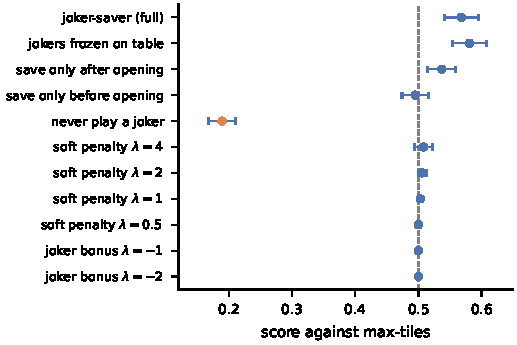
\includegraphics{figuras/tog_mecanismo.pdf}
\caption{Mechanism experiments (mean $\pm$ $95\%$ CI against max-tiles, $500$ seeds $\times$ $2$ seats each). Only the full rule, its frozen-joker control and the after-opening variant beat $0.5$; soft penalties and bonuses sit on the control, and removing the finishing exception (orange) reverses the effect.}\label{fig:mec}
\end{figure}

So the folk advice is half right: unconditional saving is far worse than not saving, and the condition ``unless it wins the game'' carries the whole effect. A held wildcard keeps an awkward hand completable; this is our reading of E3--E4, and we did not test the narrower claim about awkward last tiles.

\section{RQ3: The Metric and the Format}
\subsection{Official points}\label{sec:metric}
Everything above counts games. Official Rummikub counts tile points, and the joker-saver is precisely the policy for which the two may disagree: it ends its losses holding $0.80$ jokers, a $24$-point liability per lost game. We therefore replayed the tournament computing both metrics \emph{from the same games}, so they are perfectly paired, and added three strategies that decide when to release a joker, defined before running: \emph{saver-then-dump} (the saver, but once the pool is empty it plays the largest move even with a joker), \emph{saver-dump-near} (the saver, but it stops sparing jokers once an opponent holds three tiles or fewer) and \emph{joker-spender} (prefers moves that spend jokers; a control for the opposite extreme). Criteria were fixed on development seeds ($120$ seeds); the test seeds ($200$ seeds $\times$ $2$ seats, $18{,}000$ games) were spent once with Holm over three hypotheses.

\begin{table}[t]\centering\small\setlength{\tabcolsep}{3.5pt}
\caption{Both metrics from the same $18{,}000$ games (test seeds). Each cell is the mean against the other nine, $\pm$ $95\%$ CI over seeds; $^*$ marks a strategy added here. Points are per game and zero-sum.}\label{tab:pontos}
\begin{tabular}{@{}lccrc@{}}\toprule
Strategy & Win score & Points & Pts & Jok.\\
 & & & rank & left\\\midrule
saver-then-dump$^*$ & $0.689\pm0.017$ & $+15.0\pm1.4$ & 5 & 0.19\\
joker-saver & $0.680\pm0.017$ & $+13.3\pm1.5$ & 6 & 0.27\\
max-points & $0.639\pm0.019$ & $+19.6\pm1.0$ & 2 & 0.00\\
max-tiles & $0.633\pm0.015$ & $+19.5\pm1.0$ & 3 & 0.00\\
joker-spender$^*$ & $0.633\pm0.015$ & $+19.5\pm1.0$ & 4 & 0.00\\
saver-dump-near$^*$ & $0.622\pm0.021$ & $+19.8\pm1.1$ & 1 & 0.07\\
min-play & $0.495\pm0.025$ & $+12.6\pm1.3$ & 7 & 0.00\\
random & $0.440\pm0.020$ & $+9.7\pm1.1$ & 8 & 0.00\\
cautious & $0.160\pm0.013$ & $-26.7\pm1.8$ & 9 & 0.01\\
no-rearrange & $0.009\pm0.004$ & $-102.3\pm1.9$ & 10 & 0.01\\
\bottomrule
\end{tabular}

\end{table}
\begin{figure}[t]\centering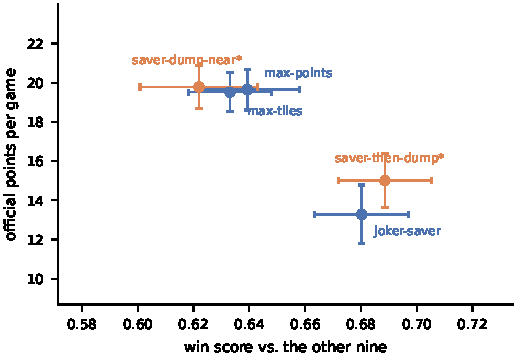
\includegraphics{figuras/tog_pontos.pdf}
\caption{The two metrics disagree, for the five strongest strategies by win score (orange: added in this section). The joker-saver is first in win score and last of the five in points. Joker-spender is omitted: it coincides with max-tiles in every comparable game.}\label{fig:pontos}\end{figure}

The ranking changes (Table~\ref{tab:pontos}, Fig.~\ref{fig:pontos}). The joker-saver is first by win score ($0.680\pm0.017$) and sixth of ten by points ($+13.3\pm1.5$), below max-tiles and max-points ($+19.5$, $+19.6$), which it beats in games won. Spearman's correlation between the two orderings is $0.64$, against $0.96$ between alternative end-of-game rules (Section~\ref{sec:rob}): the metric reorders the top far more than the rule does. Against a common field of five strategies, paired by seed, max-tiles is $+5.59$ $[+3.78,+7.39]$ points above the saver while being $-0.013\pm0.018$ below it in win score (criterion $\ge+3.0$ with a positive interval; met, $p_{\text{Holm}}<0.001$). Head-to-head the saver wins $0.573\pm0.044$ of games and still loses $5.4\pm3.1$ points per game.

The cause mirrors E4. Decomposing the saver's points against the common field: it wins $77.8\%$ of those games, and when it wins it collects $+48.0$ points, the same as max-tiles ($+47.9$) --- holding a joker buys the win, not a bigger win. When it loses it pays $-43.3$ against $-14.6$ for max-tiles, and $24$ of those $29$ extra points are the retained joker.

Intervening on the policy confirms the channel. \emph{Saver-then-dump} ends its losses with $0.64$ jokers instead of $0.80$, gaining $+2.83$ $[+1.99,+3.67]$ points \emph{and} $+0.019$ $[+0.012,+0.025]$ win score: releasing the joker once the pool is empty is free. The points gain fell short of the $+3.0$ fixed in advance, so we report it as a near miss. \emph{Saver-dump-near} releases much earlier, ends with $0.09$ jokers, pays $-17.7$ per loss, and is first of all ten in points ($+19.8\pm1.1$) while sixth in win score. \emph{Joker-spender} is inert: under max-tiles play a joker is in hand in $2.6\%$ of decisions and a choice between a joker move and a non-joker move of equal size arises in $0.1\%$, so it played identically to max-tiles in all $1{,}440$ comparable games. That is a property of the action distribution, and it explains why the joker-bonus rows of Table~\ref{tab:mec} equal the control.

\subsection{Sessions of several hands}\label{sec:session}
Rummikub is normally played as a session: several deals, points accumulated, highest total wins. Summing hands narrows the distribution around the mean, and the saver's mean is negative, so the session should amplify the effect. A session also creates information no single-hand strategy has, the accumulated balance, so we added \emph{session-adaptive}: when behind by more than one joker ($-30$ points, fixed in advance) it plays the joker-saver, maximising its chance of winning the hand; otherwise it plays saver-dump-near. Six strategies, $15$ pairs, $K=10$, both seat arrangements; development seeds ($80$ sessions per pair) then test seeds once ($120$ sessions per pair, $3{,}600$ sessions, $36{,}000$ hands), Holm over two primary criteria.

\begin{table}[t]\centering\small
\caption{Sessions of $K=10$ hands (test seeds; $120$ sessions per pair, both arrangements). Mean against the other five, $\pm$ $95\%$ CI over sessions. $^*$: not one of the original seven.}\label{tab:sessao}
\begin{tabular}{@{}lccc@{}}\toprule
Strategy & Sessions & Points & Hands\\
 & won & per session & won of 10\\\midrule
saver-dump-near$^*$ & $0.655\pm0.028$ & $+47\pm5$ & $4.76\pm0.11$\\
session-adaptive$^*$ & $0.621\pm0.028$ & $+18\pm7$ & $4.96\pm0.09$\\
max-tiles & $0.560\pm0.039$ & $+27\pm9$ & $4.77\pm0.15$\\
max-points & $0.548\pm0.041$ & $+24\pm9$ & $4.67\pm0.15$\\
saver-then-dump$^*$ & $0.329\pm0.030$ & $-49\pm9$ & $5.43\pm0.11$\\
joker-saver & $0.288\pm0.030$ & $-67\pm10$ & $5.39\pm0.11$\\
\bottomrule
\end{tabular}

\end{table}
\begin{figure}[t]\centering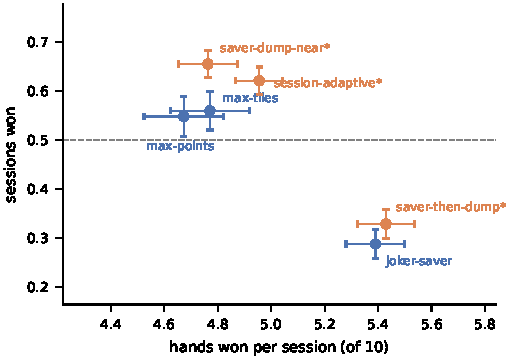
\includegraphics{figuras/tog_sessao.pdf}
\caption{Winning hands and winning sessions pull apart. The joker-saver wins the most hands per session of any strategy and the fewest sessions; releasing the wildcard before the end (orange) does the opposite.}\label{fig:sessao}\end{figure}

The inversion is complete (Table~\ref{tab:sessao}, Fig.~\ref{fig:sessao}). The joker-saver wins $5.39$ of the $10$ hands in a session, more than any other strategy, and $0.288\pm0.030$ of the sessions, fewer than any other strategy. Head-to-head against max-tiles it takes $5.53$ hands of $10$ and loses $72.5\%$ $[66.8,78.2]$ of the sessions (criterion $\ge0.55$ with the interval above $0.5$; met, $p_{\text{Holm}}<0.001$) at $-75.6\pm14.9$ points per session. The session ranking matches the per-hand \emph{points} ranking (Spearman $+0.90$) and is the exact reverse of the per-hand \emph{win} ranking (Spearman $-1.00$) on the five strategies shared by both experiments. The effect grows with session length, as the arithmetic predicts: max-tiles beats the saver in $0.558\pm0.089$ of one-hand sessions, $0.754\pm0.077$ at $K=5$ and $0.754\pm0.077$ at $K=20$, with the points margin rising from $+14$ to $+142$.

\emph{Session-adaptive} failed, in the informative direction. It loses to saver-dump-near, the fixed strategy it switches away from ($0.444$ $[0.414,0.473]$; criterion not met, and the deficit itself is significant, $p_{\text{Holm}}=0.0002$). The rule is not inert: it is behind the threshold in $26\%$ of hands. Switching to joker-saving when behind buys hands ($4.96$ per session, the most of the four strong strategies) and costs points. Chasing a deficit by saving jokers digs the hole deeper; the accumulated balance is real information that this rule turns into a loss, and we report it rather than tuning a threshold fixed in advance at one value.

\section{RQ4: Learned and Searching Agents}
We ran twenty-five agents that choose either a strategy from the menu or a concrete move (Table~\ref{tab:rl}). None beats the best heuristic. Rather than narrate each, we give the five results that carry information beyond ``no gain'': what the architecture can find, an estimate that did not replicate, the two excuses that fail, what $27\times$ more compute buys, and what per-decision credit does not.

\begin{table*}[t]\centering\small\setlength{\tabcolsep}{4pt}
\caption{Learned and searching agents, scored by game count against the two strongest heuristics ($\pm$ $95\%$ CI; seeds are per opponent, both seats). Rows marked with a signed value are paired differences against the same architecture without the change. The last row is in official points. Every row other than the two PPO rows and the official-reward row is exploratory; multiplicity is not corrected across rows.}\label{tab:rl}
\begin{tabular}{@{}llcccl@{}}\toprule
Agent & Variant & vs max-tiles & vs saver & Seeds & Status\\\midrule
\multicolumn{6}{@{}l}{\emph{Choosing a strategy from the menu}}\\
Q-learner & tabular, $6{,}000$ training games & $0.410\pm0.066$ & $0.370\pm0.060$ & 100 & below both\\
LLM & strategy selector, 600 games & $0.500$ & $0.400\pm0.060$ & 100 & plays as max-tiles\\[2pt]
\multicolumn{6}{@{}l}{\emph{Choosing a concrete move}}\\
LLM & all legal moves listed & $0.350\pm0.076$ & $0.414\pm0.072$ & 70 & below both\\
PIMC & $D{=}4$ sampled worlds & $0.542\pm0.091$ & $0.433\pm0.085$ & 60 & below saver\\
PIMC & \emph{true} world revealed & $0.508\pm0.089$ & $0.508\pm0.089$ & 60 & below saver\\
Network & REINFORCE from scratch & $0.493\pm0.029$ & $0.403\pm0.030$ & 500 & max-tiles-like\\
Network & clone of saver, untrained & $0.525\pm0.069$ & $0.455\pm0.069$ & 100 & below saver\\
Network & clone $+$ REINFORCE & $0.509\pm0.045$ & $0.487\pm0.045$ & 240 & level with both\\
Network & clone $+$ group adv.\ $K{=}4$ & $\mathbf{0.550\pm0.040}$ & $0.495\pm0.040$ & 300 & level with both\\
Network & $+$ hand-size shaping & $0.505\pm0.039$ & $0.468\pm0.041$ & 300 & no gain\\
Network & $+$ nine-opponent league & $0.546\pm0.061$ & $0.500\pm0.064$ & 40 & no gain\\
Network & $+$ rearrangement in training & $0.535\pm0.069$ & $0.510\pm0.069$ & 100 & no gain\\
Network & residual over the saver & $0.460\pm0.070$ & $0.515\pm0.070$ & 100 & never departs\\
Network & Deep Monte Carlo & $0.555$ & $0.472\pm0.068$ & 100 & below saver\\
Network & PPO (development) & $0.568$ & $0.500$ & 100 & level, not better\\
Network & PPO (held out, used once) & $0.560\pm0.056$ & $0.447\pm0.056$ & 150 & did not replicate\\
Network & $64$ hidden units & $-0.088\pm0.048$ & -- & 100 & worse than $16$\\
Network & $256$ hidden units & $+0.012\pm0.047$ & -- & 100 & no gain\\
Network & $19$ opponent features & $-0.010\pm0.021$ & -- & 120 & no gain\\
Network & $23$ tile-counting features & $-0.007\pm0.037$ & -- & 120 & no gain\\
Network & reward $=$ official points & $-5.1$ pts & -- & 100 & below max-tiles\\
\bottomrule\end{tabular}

\end{table*}

\paragraph*{The architecture can represent the mechanism; the search does not find it}
The move network scores each legal move from $15$ features (move size, jokers used, hand and pool sizes, opening status, and so on) through one hidden layer of $16$ tanh units, trained by REINFORCE against a league of heuristics, itself, and past checkpoints. Trained from scratch over $36{,}000$ games it converges to max-tiles-like play: $0.493\pm0.029$ against max-tiles, $0.403\pm0.030$ against the saver, going out with a joker in $2.9\%$ of games against the saver's $41\%$. Supervised cloning of the saver on $10{,}587$ of its decisions reaches $82\%$ agreement on held-out decisions and reproduces the mechanism ($70\%$ of its wins end with a joker), which shows the features suffice to express the rule. What the from-scratch run lacked was the search for it. The candidate explanation, credit assignment (one reward per hand, after roughly sixty decisions), did not hold when tested (Section~\ref{sec:passo}), and its premise was wrong in one respect: a real choice between playing and keeping a joker arises in $17.3\%$ of decisions ($4{,}024$ sampled) and keeping it always costs tiles, so it is a recurring trade-off, not a rare end-of-hand event.

\paragraph*{One positive estimate did not replicate}
Cloning the saver and refining it gave, on the first training seed, $0.605$ against max-tiles, the only number that appeared to beat both heuristics. Two further seeds gave $0.509\pm0.045$: a favourable draw, selected by looking. Group-relative advantages \cite{shao2024} with four games per deal reach $0.550\pm0.040$ against max-tiles ($p=0.014$ uncorrected), the only interval here excluding $0.5$ against it, read cautiously. Grouping stabilises the mechanism ($59$--$66\%$ of wins end with a joker against $14$--$43\%$ without it). PPO shows the same pattern at larger scale: $0.500$ on development seeds, $0.447$ held out.

\paragraph*{Neither hidden information nor the reward is the binding constraint}
Giving the determinised search the \emph{true} world leaves it at $0.508\pm0.089$ against the saver, so perfect information does not lift this search above the heuristic. Retraining with reward $=\text{points}/60$ from the same clones, networks learn what the heuristics say is worth points ($0.22$ jokers in hand against the control's $0.28$, $58\%$ of wins ending with a joker against $69\%$, $-33.2$ points per loss against $-38.7$) but gain only $+1.7$ $[-0.7,+4.1]$ over the control, short of the $+3$ fixed in advance, and remain $5.1$ points \emph{below} max-tiles on the metric they optimise: the official reward teaches a one-line heuristic, worth $4.5$ points.

\paragraph*{Scaling the budget $27\times$ changes the mechanism, not the ranking}\label{sec:orcamento}
Every row of Table~\ref{tab:rl} trains on $7{,}200$ games. We repeated the best recipe changing \emph{only} the budget: $192{,}000$ games per seed, three seeds, $9.9$~h on six cores, criteria fixed in advance. Against the joker-saver the scaled agent scores $+4.69$ $[+2.10,+7.28]$ official points, the first learned agent here whose interval excludes zero against the champion on the metric the rules define. Its gain over the same recipe at the old budget, $+2.83$ $[-0.84,+6.51]$ on $150$ hands and short of the $+5$ we required, is $+3.57$ $[+2.24,+4.90]$ on $1{,}200$ fresh hands (seeds $300{,}000$+), positive for each of the three training seeds ($+1.8$, $+4.4$, $+4.5$).

The mechanism inverts the usual story: the scaled agent \emph{wins fewer hands} than its own control ($0.390$ against $0.487$) yet scores more points, because it loses far more cheaply ($-18.1$ against $-42.5$ per loss). In defeat it ends with $2.78$ tiles and $0.011$ jokers, against $4.31$ and $0.604$: it learned to release the joker and empty its hand \emph{before} losing, the policy Section~\ref{sec:metric} says the official metric rewards, found by search rather than written by us. Training return saturated near iteration $450$ of $4{,}000$: $27\times$ the games bought about $3.6$ points and then nothing, so budget is not the explanation for the nulls.

\emph{Is it then the best player? On average it trails the best by about a point.} Entered in the thirteen-competitor common-field tournament of Section~\ref{sec:metric} ($9{,}360$ games, seeds $270{,}000$+), the network ranks \emph{first} in official points ($+16.96$ against max-tiles' $+15.60$), but the paired comparison on identical hands against the same nine common opponents is $-1.69$ $[-3.70,+0.31]$: the ranking is an artefact of each agent facing a slightly different field. Head-to-head over $1{,}200$ fresh hands the three networks average $-1.15$ $[-1.63,-0.67]$ points and $0.472\pm0.012$ of hands, but one is indistinguishable from max-tiles ($-0.10$ $[-0.84,+0.65]$) and another loses $2.59$; that interval conditions on these three networks (with the seed as the unit, $[-4.35,+2.06]$), so we replicate with thirty seeds below. What survives is that it beats the joker-saver in points head-to-head, $+5.59$ $[+1.42,+9.75]$, the only learned agent here to do so.

\paragraph*{Per-decision credit does not lift the agent either}\label{sec:passo}
Every result above trains on one scalar per hand, so the roughly sixty decisions of a hand share one credit, the explanation we had offered for the nulls. We gave each decision its own reward by potential shaping \cite{ng1999}, $r_t=\Phi(s_{t+1})-\Phi(s_t)$ with $\Phi=-(\text{tile points}+30\cdot\text{jokers in hand})/60$, so releasing a joker is worth $+0.5$ at the step it happens; the sum telescopes to a policy-independent constant, so the optimal policy is unchanged. Treatment and control share the clone and differ only in this flag (three seeds each, $48{,}000$ games per seed; criterion $\ge+3$ points, interval excluding zero). It did not help: $-2.12$ $[-5.43,+1.20]$ points against its own control (by seed $-0.3$, $-0.2$, $-5.9$) and $-1.94\pm1.47$ against max-tiles (control $-0.12\pm1.36$). The intervention was verified as applied (L2 distance between treatment and control weights $1.59$); the held-out seeds were not spent. Either $\Phi$ rewards emptying the hand, which max-tiles already does, and pushed the network towards greedy play, or the budget is short for a dense signal, or credit assignment was not binding.

\paragraph*{Session-aware training does not help, and thirty training seeds settle what three could not}\label{sec:sessrl}
Every agent above trains and is scored hand by hand, although Section~\ref{sec:session} argues the session is the format that matters. A network that sees the running balance has a lever no policy of ours has: an underdog gains from variance (at the same mean of $-1.15$, raising the per-hand standard deviation from $19.6$ to $33$ lifts the ten-hand session win probability from $0.426$ to $0.456$ under a normal model). We added two inputs, the balance and the share of hands left, zero-initialised so that the network starts unchanged, and trained it on a potential over the probability of winning, $V(s,h)=\Phi(s/(\sigma\sqrt h))$ with $\sigma=30$, whose per-hand differences telescope exactly to the session outcome. The control has the same inputs, sessions and opponents and is rewarded in points per hand, so the pair isolates the reward. A first run with three seeds per arm gave $-0.014$ $[-0.030,+0.002]$, but networks within one arm ranged from $0.36$ to $0.49$ in session win rate, even in the arm with no session training, and the difference by seed was $+0.110$, $-0.067$, $-0.086$: that interval resolved three networks, not the procedure.

We therefore repeated the pipeline with thirty independent training seeds per arm (own clone, training hands and evaluation; $t$ intervals with the seed as the unit, criteria fixed in advance, Holm over four hypotheses; $48{,}000$ games per seed, $4{,}800$ sessions for the session arms). The $48{,}000$-game recipe beats the joker-saver by $+5.72$ $[+5.12,+6.31]$ points per hand and gains $+1.84$ $[+0.74,+2.95]$ over the $7{,}200$-game one (Holm $p=0.005$), about half the three-network estimate. Against max-tiles it loses $0.89$ $[0.51,1.26]$ points per hand (Holm $p=0.0002$), and $5$ of $30$ networks reach parity. The session-trained agent wins $0.472$ $[0.449,0.495]$ of sessions against max-tiles and its control $0.461$ $[0.439,0.482]$. Their paired difference is $+0.011$ $[-0.021,+0.044]$: by our pre-set $\pm0.04$ band it is inconclusive, by $0.004$, since it excludes a gain above about four points but not a smaller one. The mechanism is absent: pooling networks, the agent seems to keep a joker more often when behind ($1.6\%$ of hands) than ahead ($1.3\%$), but per network the difference is $-0.0006$ $[-0.0028,+0.0017]$, as for the control (post hoc). Seed spread falls with budget (standard deviation between networks against max-tiles: $2.05$ points per hand at $7{,}200$ games, $1.01$ at $48{,}000$) but session win rates still range from $0.27$ to $0.57$.

\paragraph*{A language model as decision-maker}
A commercial System One model, in two roles: as a strategy selector over $600$ games it chose max-tiles in $84\%$ of decisions and ``draw'' in $16\%$, never the joker-saver, scoring $0.500$ against max-tiles (it \emph{is} max-tiles here). Given every legal move instead, with each option's consequence computed in code, it scored $0.350\pm0.076$ against max-tiles, playing a joker in $3$--$4\%$ of moves. The prompt stated the rules but no strategy advice. Total spend US\$$3.1$.

\section{Robustness}\label{sec:rob}
Five checks support the game-count results of Sections~\ref{sec:mech} and~\ref{sec:metric}; all are reported in full in the supplement.

\textbf{End-of-game rule.} Our main experiments score a stalled pool as a draw ($16.3\%$ of games). Replaying the same $3{,}360$ games under the official tie-break and under fewest-tiles leaves the ranking and the mechanism unchanged (Spearman $0.96$ for both; saver's lead $0.755$, finishing-tile ablation $0.164$). Only the bottom moves: no-rearrange falls from $0.271$ to $0.010$, since $54\%$ of its games ended in pool exhaustion, which had flattered it.

\textbf{Rearrangement cap.} The $128$-plan cap is reached in $9.9\%$ of decisions, $73\%$ of games. Replaying with caps of $512$, $2{,}048$ and $4{,}096$ leaves the ranking identical and \emph{increases} the saver's edge ($0.525\to0.625$), so truncation understates the effect; an offline oracle re-enumerating $383$ capped states found a play with more tiles in $4.2\%$ of them, always by one.

\textbf{A wider menu.} A $12$-strategy league ($66$ pairs, $10{,}560$ games) keeps the saver first by mean score and Bradley--Terry strength, though three joker-timing variants are not separable from it. The finishing-joker pattern reappears: $59$--$62\%$ of the saver's wins and its closest variant's end with a joker, against $0$--$18\%$ for the others.

\textbf{More players.} At three players the saver keeps a smaller edge ($0.374$ against chance $0.333$); at four it is at chance ($0.249$). The finishing-joker ablation still collapses at three players ($0.159$). Networks retrained with a curriculum over tables of two to ten players gain $+0.04$ to $+0.06$ at four, six and ten players on held-out seeds, and one trained \emph{only} on six-to-ten-player tables is indistinguishable from it, so what matters is having seen large tables.

\textbf{A paired tournament against the strong field, and a win-reward scaling test.} A fixed field of six strong strategies (max-tiles, max-points, the joker-saver, three joker-timing variants), the same for every candidate and table size, avoids the artefact of Section~\ref{sec:orcamento}. \emph{Saver-then-dump} leads at two players ($0.5345\pm0.0113$, $+0.0594$ over max-tiles); the margin shrinks to $+0.0362$ at three and is a resolved null at four ($-0.0005$ $[-0.0082,+0.0072]$, band $\pm0.02$). Trained networks never separate from the best heuristic at any table size. We also scaled a \emph{win}-reward network from a clone of saver-then-dump at $7{,}200$, $48{,}000$ and $192{,}000$ games. The clone trails it by $-0.070$; $7{,}200$ games close most of that ($-0.004$); more training is \emph{worse}: $-0.034$ at $48{,}000$, $-0.094$ $[-0.139,-0.049]$ at $192{,}000$, below the clone. The reward is not the obstacle --- it moves the network the right way at the small budget --- the training opponents are: every variant trains against the same seven weaker heuristics, never saver-then-dump, and win rate against that menu keeps climbing while win rate against the strong field falls after an early peak.

\textbf{An independent opponent.} All matches above are between policies we wrote, so we also played third-party code: an open-source Rummikub solver \cite{rummikubsolver} built on the integer-programming formulation of \cite{denhertog2006}, whose default rule set matches ours exactly. Wrapped in the obvious greedy player (best placement if it melds anything, otherwise draw) it wins $0.040$ $[0.015,0.064]$ of two-player games against the saver and essentially none with three or four players: it melds $13$ tiles per game and draws about $40$ times, where the saver melds $21$. Our trained networks beat it in essentially every game: optimal per-turn placement is not a policy.

\section{Discussion}\label{sec:disc}
\paragraph*{On Rummikub}
The simulation supports a narrow, mechanistic answer to what wins a single hand by game count: play the biggest legal move, but keep jokers until one lets you go out. Three competing explanations fail and the finishing-tile intervention reverses the effect, but the practical advice inverts with the format. Under the scoring printed in the rules, keeping a joker costs about six points a hand against simply playing the most tiles, and over a session the same policy wins the most hands and the fewest sessions. The mechanism is one object seen from two sides: a held wildcard is a bet that pays a win and charges $30$ points when it fails, and which side dominates is decided by the scoring rule and the format, not by the game. Releasing the joker before the end improves both points and sessions, so the frontier is not a strict trade-off everywhere. The advantage is also a property of the table: against a fixed strong field it shrinks from two to three players and disappears at four, consistent with fewer turns in which a held joker can still pay off.

\paragraph*{On measurement}
The methodological point does not depend on Rummikub. Game count is the cheap, conventional metric; points over a session is the one the rules define. On our menu they were \emph{anti-correlated}: a per-hand win rate of $0.573$, the kind of margin routinely reported as an improvement, corresponded to losing three sessions in four, and the session ranking reversed the per-hand win ranking. No number of additional seeds on the cheap metric would have revealed this, unlike the statistical-reliability concerns of \cite{agarwal2021}: more runs sharpen an estimate of the wrong quantity. When a game defines a score, measure it; when it is played in sessions, simulate sessions; where proxy and objective disagree, report both.

\paragraph*{On the learning results}
Twenty-five agents fail to beat the best heuristic under both metrics. Within one family (a $273$-parameter network over $15$ features, Monte Carlo policy gradient), separate experiments remove the capacity to express the saver's rule, hidden information, the reward, the training budget, per-decision credit (Section~\ref{sec:passo}) and session state (Section~\ref{sec:sessrl}). What is left is the baseline's strength, the observation, and \emph{who the agent trains against}: scaling the win reward keeps improving against its own league of seven weaker heuristics while getting worse against the strong field that includes the champion, which it never faces in training --- not evidence against RL, since the same recipe moves the network the right way at a smaller budget, but evidence that curriculum and evaluation target different objectives. The leading hypothesis is that max-tiles and saver-then-dump are hard to beat on this menu; thirty seeds show this family trails max-tiles by about a point per hand and three points of session win rate. The contrast with IRumAI \cite{mohan2026} ($53.9\%$ against a strong search baseline in Indian Rummy, same clone-then-policy-gradient outline) points to scale, observation design, and a training league with the strongest heuristics, as where we would look next.

\section{Limitations}\label{sec:lim}
\begin{itemize}\itemsep0pt
\item \textbf{Menu.} ``Best'' means best of sixteen hand-written strategies; stronger policies may exist. The move network has a $16$-unit hidden layer and hyper-parameters were not tuned; only one value each of the learning rate, group size, shaping weight and adaptive threshold was tried. The budget experiment scaled games, not capacity or hyper-parameters. The shaping experiment tried one potential, $-$(hand liability), at one budget; one built on formable melds is a different experiment we did not run, nor did we test a meld-aware observation.
\item \textbf{Joker identity on the table.} Officially a melded joker must keep representing the same tile unless the player supplies that tile. Our engine stores a joker as a value-free tile and validates only the final sets, so a rearrangement can silently change what a table joker represents. Our frozen-joker ablation is stricter than the official rule and the default more permissive, so the true rule lies between two conditions we measured. Every main result concerns jokers, so this is the fidelity gap we would close first.
\item \textbf{Scope of the metric results.} The dual-metric tournament and the sessions are two players only, and the sessions use $K=10$ (with $K\in\{1,5,20\}$ in one cell) and model hands as independent apart from the accumulated balance. The mechanism ablations, the league and the larger tables were run on game count. The $192{,}000$-game win-reward networks trained against the same seven-heuristic menu as every other agent in Table~\ref{tab:rl}, excluding the champion they are evaluated against; we did not retrain against a league that includes it.
\item \textbf{Statistics.} Normal-approximation intervals over seeds; Holm families cover the mechanism table, the league and each confirmatory experiment separately. Table~\ref{tab:rl} is uncorrected across rows, and the three training seeds of each learned variant share deals, so pooled intervals are optimistic in the sense of \cite{agarwal2021}. Only the $48{,}000$-game hand recipe and the session arms were replicated with thirty seeds (Section~\ref{sec:sessrl}).
\item \textbf{Simulation only.} No human players, and the language-model results are one prompt and one pinned model version.
\end{itemize}

\section{Conclusion}
Among seven interpretable Rummikub strategies, hoarding wildcards until one can end the hand wins the most hands ($0.726\pm0.027$), and an intervention on that single exception reverses the advantage ($0.568\to0.189$). Scored by the tile points the rules define, the same policy falls to sixth of ten, $5.6$ points per hand below simply playing the most tiles; played as sessions of ten hands it wins the most hands of any strategy and the fewest sessions, losing $72.5\%$ of sessions to max-tiles, and the session ranking is the exact reverse of the per-hand win ranking. A fixed strong field confirms the advantage shrinks from two to three players and vanishes at four. Twenty-five learned and searching agents, including PPO, Deep Monte Carlo, a search given the true hidden hands, training on the official reward, a $27\times$ larger budget, per-decision potential shaping, session-aware training, and a $192{,}000$-game win-reward recipe, fail to beat the best heuristic under either metric; the win-reward recipe gets \emph{worse} with more training because it never trains against that heuristic. The largest points-budget agent is the first to beat the champion in points, by winning fewer hands and losing more cheaply, yet over thirty independent training seeds a $48{,}000$-game recipe trails the strongest heuristic by $0.89$ $[0.51,1.26]$ points per hand. The strategy result is specific to this simulator and menu; the measurement result is not: the conventional metric and the one the rules define were anti-correlated here.

\section*{Reproducibility}
Code, per-game records for every table, and all analysis scripts are in the anonymised supplementary repository, \repoanon. Every experiment is a subcommand of one entry point; each confirmatory experiment fixed its criterion and seed ranges before running.

\footnotesize
\begin{thebibliography}{99}
\setlength{\itemsep}{0pt}\setlength{\parskip}{0pt}
\bibitem{vanrijn2016} J.~N. van Rijn, F.~W. Takes, and J.~K. Vis, ``The complexity of Rummikub problems,'' \emph{arXiv:1604.07553}, 2016, (BNAIC 2015).
\bibitem{denhertog2006} D.~den Hertog and P.~B. Hulshof, ``Solving Rummikub problems by integer linear programming,'' \emph{The Computer Journal}, vol.~49, no.~6, pp.~665--669, 2006.
\bibitem{feijen2023} R.~Feijen, ``Counting winning hands in Rummikub,'' B.Sc. thesis, LIACS, Leiden University, 2023.
\bibitem{wekken2025} M.~van der Wekken, ``Algorithms for Rummikub puzzles,'' B.Sc. thesis, LIACS, Leiden University, 2025.
\bibitem{kotnik2003} C.~Kotnik and J.~K. Kalita, ``The significance of temporal-difference learning in self-play training: TD-Rummy versus EVO-Rummy,'' in \emph{Proc. 20th Int. Conf. Machine Learning (ICML)}, 2003, pp.~369--375.
\bibitem{zha2021} D.~Zha, J.~Xie, W.~Ma, S.~Zhang, X.~Lian, X.~Hu, and J.~Liu, ``DouZero: Mastering DouDizhu with self-play deep reinforcement learning,'' in \emph{Proc. ICML}, 2021.
\bibitem{li2020} J.~Li \emph{et al.}, ``Suphx: Mastering Mahjong with deep reinforcement learning,'' \emph{arXiv:2003.13590}, 2020.
\bibitem{balla2024} M.~Balla, G.~E.~M. Long, J.~Goodman, R.~D. Gaina, and D.~Perez-Liebana, ``PyTAG: Tabletop games for multi-agent reinforcement learning,'' \emph{arXiv:2405.18123}, 2024.
\bibitem{rudolph2025} M.~Rudolph \emph{et al.}, ``Reevaluating policy gradient methods for imperfect-information games,'' \emph{arXiv:2502.08938}, 2025.
\bibitem{schulman2017} J.~Schulman, F.~Wolski, P.~Dhariwal, A.~Radford, and O.~Klimov, ``Proximal policy optimization algorithms,'' \emph{arXiv:1707.06347}, 2017.
\bibitem{shao2024} Z.~Shao \emph{et al.}, ``DeepSeekMath: Pushing the limits of mathematical reasoning in open language models,'' \emph{arXiv:2402.03300}, 2024.
\bibitem{ng1999} A.~Y. Ng, D.~Harada, and S.~Russell, ``Policy invariance under reward transformations: Theory and application to reward shaping,'' in \emph{Proc. ICML}, 1999, pp.~278--287.
\bibitem{mohan2026} V.~Mohan \emph{et al.}, ``IRumAI: Reinforcement learning for Indian Rummy,'' \emph{arXiv:2606.21975}, 2026.
\bibitem{frank1998} I.~Frank and D.~Basin, ``Search in games with incomplete information: A case study using bridge card play,'' \emph{Artificial Intelligence}, vol.~100, no.~1--2, pp.~87--123, 1998.
\bibitem{long2010} J.~Long, N.~R. Sturtevant, M.~Buro, and T.~Furtak, ``Understanding the success of perfect information Monte Carlo sampling in game tree search,'' in \emph{Proc. AAAI}, 2010.
\bibitem{cowling2012} P.~I. Cowling, E.~J. Powley, and D.~Whitehouse, ``Information set Monte Carlo tree search,'' \emph{IEEE Trans. Computational Intelligence and AI in Games}, vol.~4, pp.~120--143, 2012.
\bibitem{agarwal2021} R.~Agarwal, M.~Schwarzer, P.~S. Castro, A.~Courville, and M.~G. Bellemare, ``Deep reinforcement learning at the edge of the statistical precipice,'' in \emph{Proc. NeurIPS}, 2021.
\bibitem{holm1979} S.~Holm, ``A simple sequentially rejective multiple test procedure,'' \emph{Scandinavian Journal of Statistics}, vol.~6, pp.~65--70, 1979.
\bibitem{rummikubsolver} ``Rummikub solver library,'' open-source software under the MIT License, 2025. Repository cited in the supplementary material to preserve anonymity.
\bibitem{pagat2024} J.~McLeod, ``Rummikub,'' \emph{Card Games website}, accessed Oct.~2026. [Online]. Available: \url{https://www.pagat.com/rummy/rummikub.html}
\end{thebibliography}

\end{document}
